\documentclass[letterpaper,twocolumn,10pt]{article}
\usepackage[margin=.95in]{geometry}
\usepackage{times}
\usepackage{graphicx}
\usepackage{xcolor}
\usepackage{tikz}
\usepackage{makecell}
\usepackage{hyperref}
\usepackage{xspace}

\sloppy

\title{You Can't Corrupt What You Couldn't See: Redesign IoT OS with Rust}
\author{ \\ Computer Science @ UC Davis}

\author{
  Yuyang(Peter) Rong\\
  PtrRong@ucdavis.edu
  \and
  Haitian Chen \\
  HtiChen@ucdavis.edu
  \and
  Yubo Wang \\
  YboWang@ucdavis.edu
  \and
  Jingyuan Li \\
  AjyLi@ucdavis.edu
}

\date{}

\pagestyle{plain}
\pagenumbering{arabic}

\newcommand{\todo}[1]{\textcolor{red}{#1}}
\newcommand{\ritos}{RITOS\xspace}
\newcommand{\rpi}{\textit{Raspberry Pi}\xspace}
\newcommand{\rpis}{\textit{Raspberry Pi}s\xspace}

\begin{document}

\maketitle

\begin{abstract}
\todo{
    This is my abstract.  I usually keep these short and too the point
    (around 200-300 words).  You don't have to cite anything -- in fact it
    is considered poor form to cite things in your abstract -- but you do
    need to give the reader an idea about what you did.  It is also a good
    idea to put numbers in your abstract.
}
\end{abstract}

\section{Introduction}

\todo{1-2 paragraphs about what problem you are solving and why it is important.}

Internet of Things(IoT) has posted new security threats since its first appearance. 
It is estimated that "by 2020, More Than 25 Percent of Identified Attacks in Enterprises Will Involve IoT"\cite{gartner2016gartner}.

\todo{1-2 paragraphs about how other people have solved this problem and how they fall short.}

There have been efforts on how to secure IoT devices from a system perspective like \textit{The Seven Properties}\cite{hunt2017the} proposed by Galen Hunt.
People have also worked on how to create new systems including SPIN\cite{hesselman2017spin} and Tock\cite{levy2017tock}.

\todo{1 paragraph (optional) what is difficult about this problem.}

\todo{1-2 paragraphs about your plan on why it is better than current approaches.}

In this work, we present the Rust IoT Operating System(RITOS).
We plan to write a new IoT OS from scratch using Rust in the first stage.
Rust is a programming language designed to do system programming and has safety mechanisms designed in the core language.
It has powerful compile-time checks that find most of the common memory bugs.
Therefore we can guarantee that there is a minimum number of bugs as most of them can be opt-out at compile time. 
Another advantage of our customized OS is that we can reduce the trusted computing base(TCB) to a small LOC.

In the second stage, we would re-organize the architecture of the devices.
We believe that \textit{You can't corrupt invisible things}.
Therefore we arranged devices so that most of the \textit{Slave devices} are invisible from the perspective of the public network.
Machines outside this IoT network can only talk to the \textit{Master device}.
We added extra authentication before a user can talk to the master device.

\todo{1 paragraph to summarize results, or for your project proposals summarize your anticipated results.}

In the end, we would build this network. 
We would use 2 Raspberry Pis to mimic a master device and a slave device. 
We as the user would use a shell from our Laptop to issue commands(Since we are not interested in writing a fancy UI).
\section{Design}

\begin{figure*}[h]
    \centering
    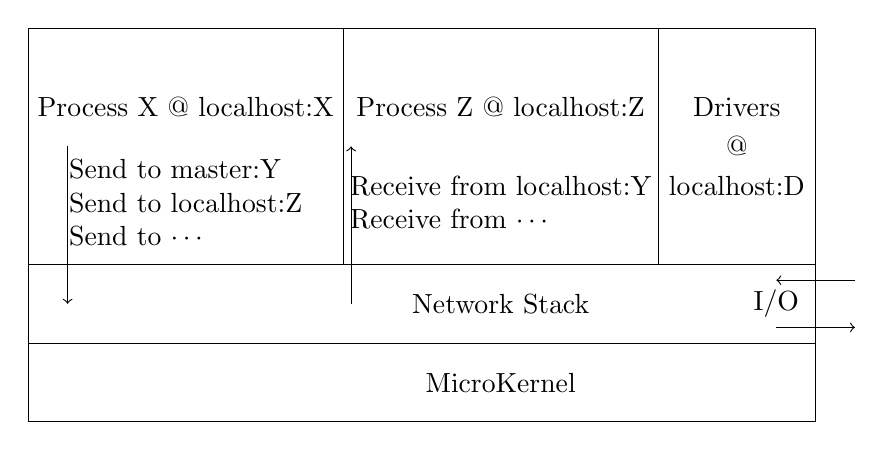
\begin{tikzpicture}

        \begin{scope}[shift={(1,1)},local bounding box=IoTOS]
            \draw (0,0) rectangle (10, 5);
            \draw (0,1) rectangle (10, 2);
            \draw (0,2) rectangle (4, 5);
            \draw (4, 2) rectangle (8, 5);
            
            \node at (6, 0.5) {MicroKernel};
            \node at (6, 1.5) {Network Stack};
            
            \node at (2, 4) {Process X @ localhost:X};
            \node at (2, 2.75) {\makecell[l]{Send to master:Y \\ Send to localhost:Z  \\ Send to $\cdots$}};
            \draw[->] (0.5, 3.5) -- (0.5, 1.5);

            \node at (6, 2.75) {\makecell[l]{Receive from localhost:Y  \\ Receive from $\cdots$}};
            \draw[->] (4.1, 1.5) -- (4.1, 3.5);

            \node at (6, 4) { Process Z @ localhost:Z };
            \node at (9, 4) { Drivers };
            \node at (9, 3.5) { @ };
            \node at (9, 3) { localhost:D };

            \node at (9.5, 1.5) {I/O};
            \draw[->] (9.5, 1.2) -- (10.5, 1.2);
            \draw[->] (10.5, 1.8) -- (9.5, 1.8);
            
        \end{scope}
        
        IoTOS
\end{tikzpicture}
\end{figure*}
\section{Implementation}

We would take down the parts and implement this system step by step.

As the first step we would implement IoTOS on \rpi. 
The mile stone for the first stage is to ask IoTOS to host two processes and for them to be able to communicate through network APIs.
Here, to make things easier we would not implement encryption nor authantication yet.

The second part would be to implement the drivers for LED light, slave process and master process.
By the end of this part we would be able to connect two \rpis. 
They should be able to identify who's slave and who's master according to configuration and master device is able to open a LED  connected to slave device.

The thrid part would be to secure all the things we have implemented.
One would be to force devices communite through HTTPS, another would be to ask every entity in this network, including user himself, to proof them not malicious through authtication methods.

\section{Related Work}

\subsection{Operating Systems with Rust}

The browser has become de facto operating systems nowadays.
Servo\cite{Servo} is a Rust version of the browser engine designed by Mozilla.
Yet, the browser engine is not a good fit for IoT as the code base tends to be huge.

There have also been attempts to write a new OS from scratch using Rust.
Redox\cite{Redox} is a microkernel-based OS, it is highly finished and useable with POSIX API implemented in Rust and a GUI for desktop users.
Some individuals are also writing personal blogs\cite{OsPhil} to write an OS from scratch step by step, yet it is still not finished and only runs in QEMU. 

Few attempts have been made on writing Rust based embedded OS, but none of them targets any specific security issues as we do.
Tock\cite{levy2015ownership, levy2017tock, levy2017multiprogramming} is an embedded operating system designed for running multiple concurrent, mutually distrustful applications on Cortex-M and RISC-V based embedded platforms.
There have been community efforts to deliver tutorials through Github.com\cite{rpi-os-t0, rpi-os-t1}
Sergio also finished an IoT OS framework in Rust\cite{cs140e} and leave the rest to the student as the course project in CS140e at Stanford.

\subsection{IoT Security}

In an IoT system, different IoT devices connect and interact with each other through the network, which makes it vulnerable when devices are directly exposed. 
Common security issues of the IoT system are divided into three categories: low-level issues, intermediate-level security issues, and high-level security issues.

Low-level security is based on vulnerabilities in the physical layer of network and hardware layers of devices. 
For example, jamming attacks create illegal radio signals to disturb normal wireless communication between IoT devices\cite{xu2005feasibility,noubir2003low}. 
In addressing spoofing attack, adversarial devices masquerade as normal devices to spread malicious network packets\cite{chen2007detecting}.

Intermediate-level security deals with transportation layer security, such as the routing mechanism. 
RPL attack is based on the vulnerability of the routing protocol for low-power and lossy networks(RPL)\cite{dvir2011vera}. 
Attackers may compromise devices in a network to leak private data.

High-level security concerns about vulnerable applications and interfaces on IoT devices. 
Many IoT management web interfaces are susceptible to attacks\cite{owasp2016url}. 
Insecure middleware for data process and behavior analysis may cause security issues such as MitM attack\cite{conzon2012virtus,levy2015ownership}. 
And insecure firmware may also throw a great threat to data privacy\cite{owasp2016url}.

Some research aims to develop trustworthy standards of security IoT devices and software. 
\textit{The Seven Properties}\cite{hunt2017the} come up with several required properties of highly secure devices, which cover many significant aspects of IoT security, such as trusted computing, authentication, failure reporting, etc.

SPIN\cite{hesselman2017spin} provides a set of a complete solution for in-home network security. 
It detects many common networks issue, including DoS attack, privacy data leaking, and device compromising.


\bibliographystyle{abbrv}
\bibliography{main}
\end{document}
